\chapter{Results and Discussions}
\section{Results}



\subsection{Descriptive Statistics}

\begin{figure}[ht]
    \centering
    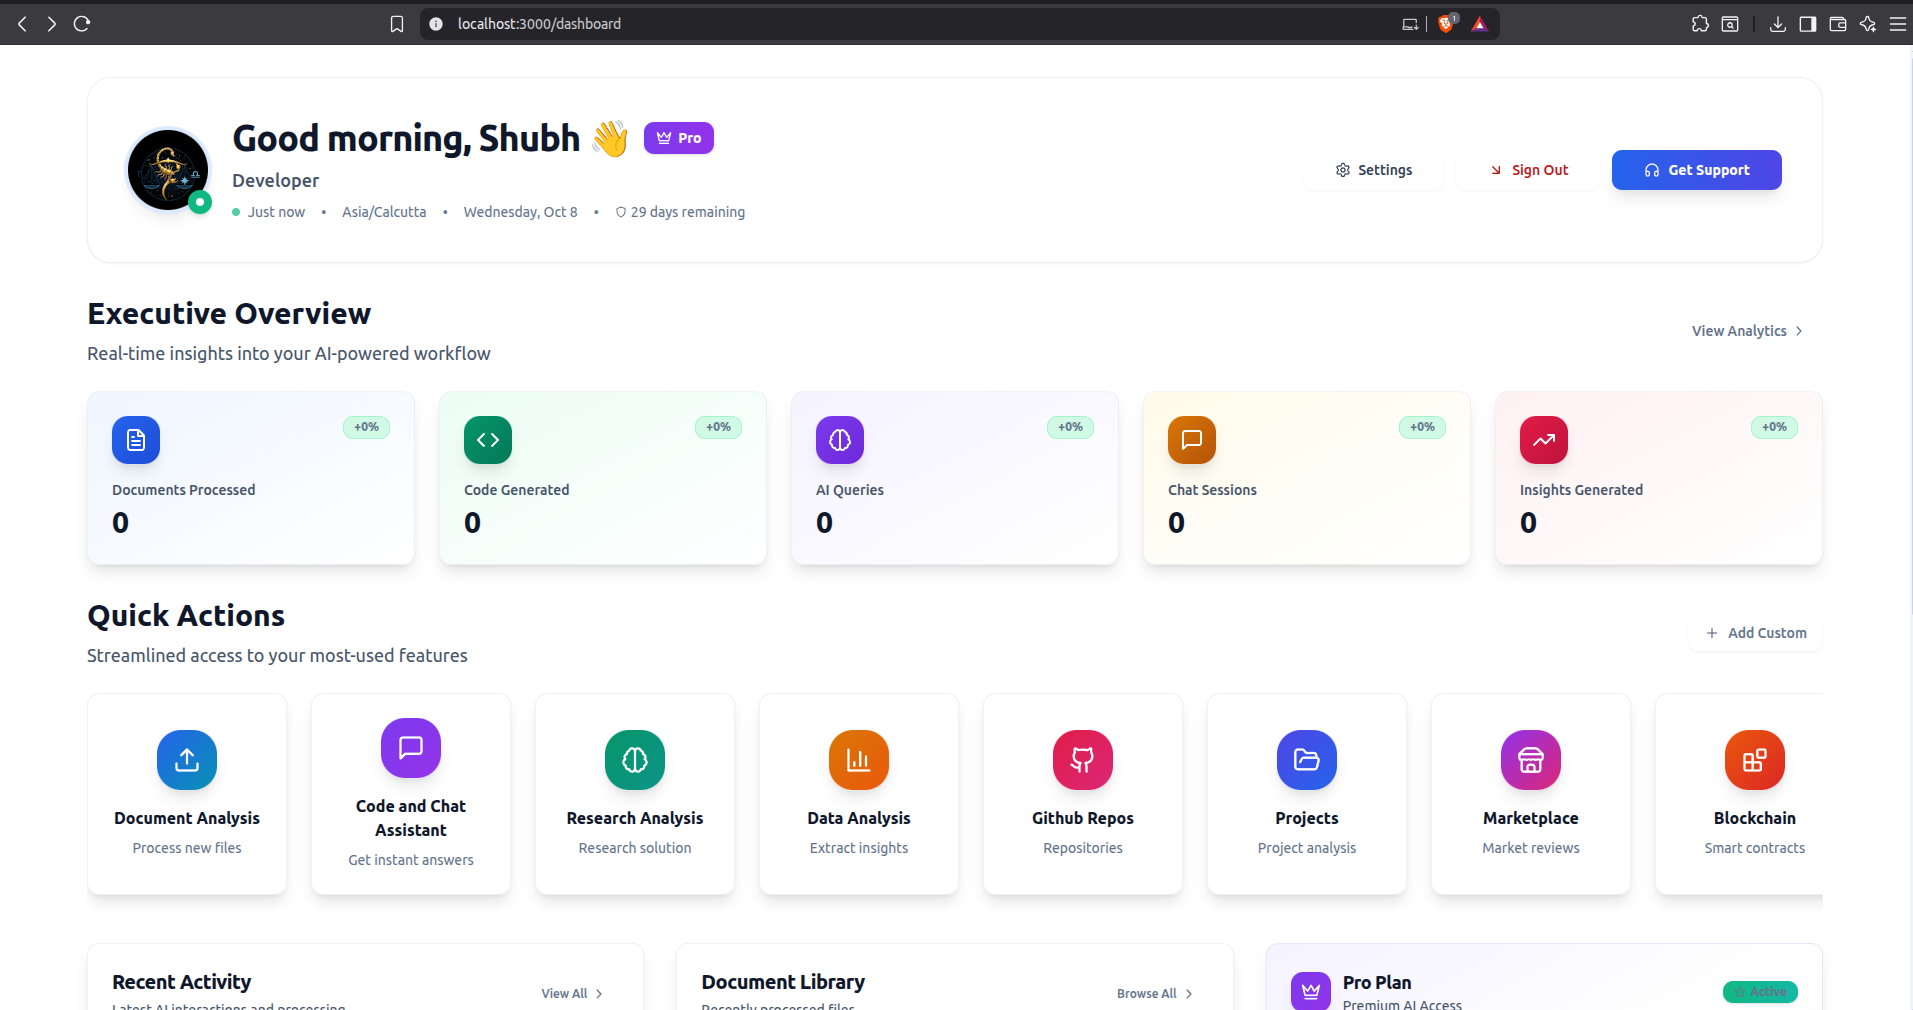
\includegraphics[width=0.75\textwidth]{images/Screenshot from 2025-10-08 00-21-40.png}
    \caption{Dashboard.}
    \label{fig4.1.1:single1}
\end{figure}

\begin{figure}[h!]
    \centering
    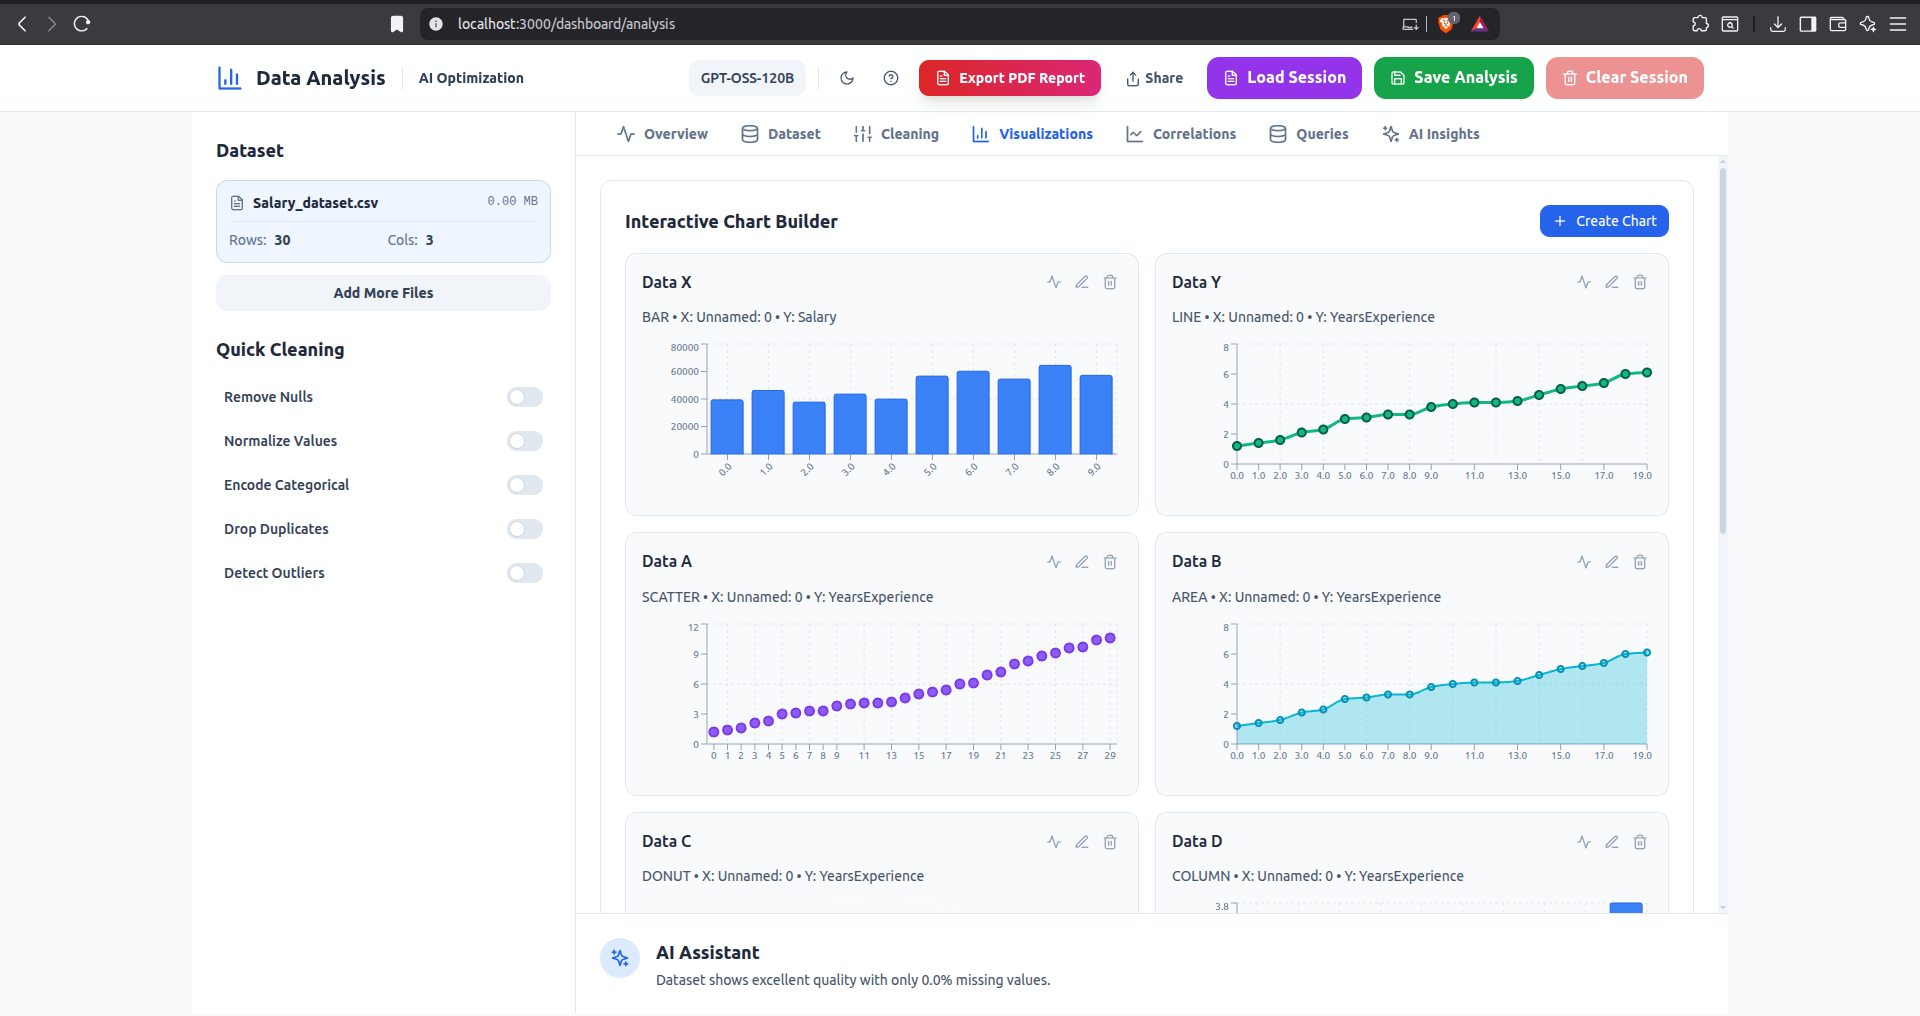
\includegraphics[width=0.85\linewidth]{images/Screenshot from 2025-10-07 23-58-57.png}
    \caption{Data Analysis}
    \label{fig4.1.2:dataanalysis}
\end{figure}

\vspace{3em} % <-- adds a small gap between figures

\begin{figure}[h!]
    \centering
    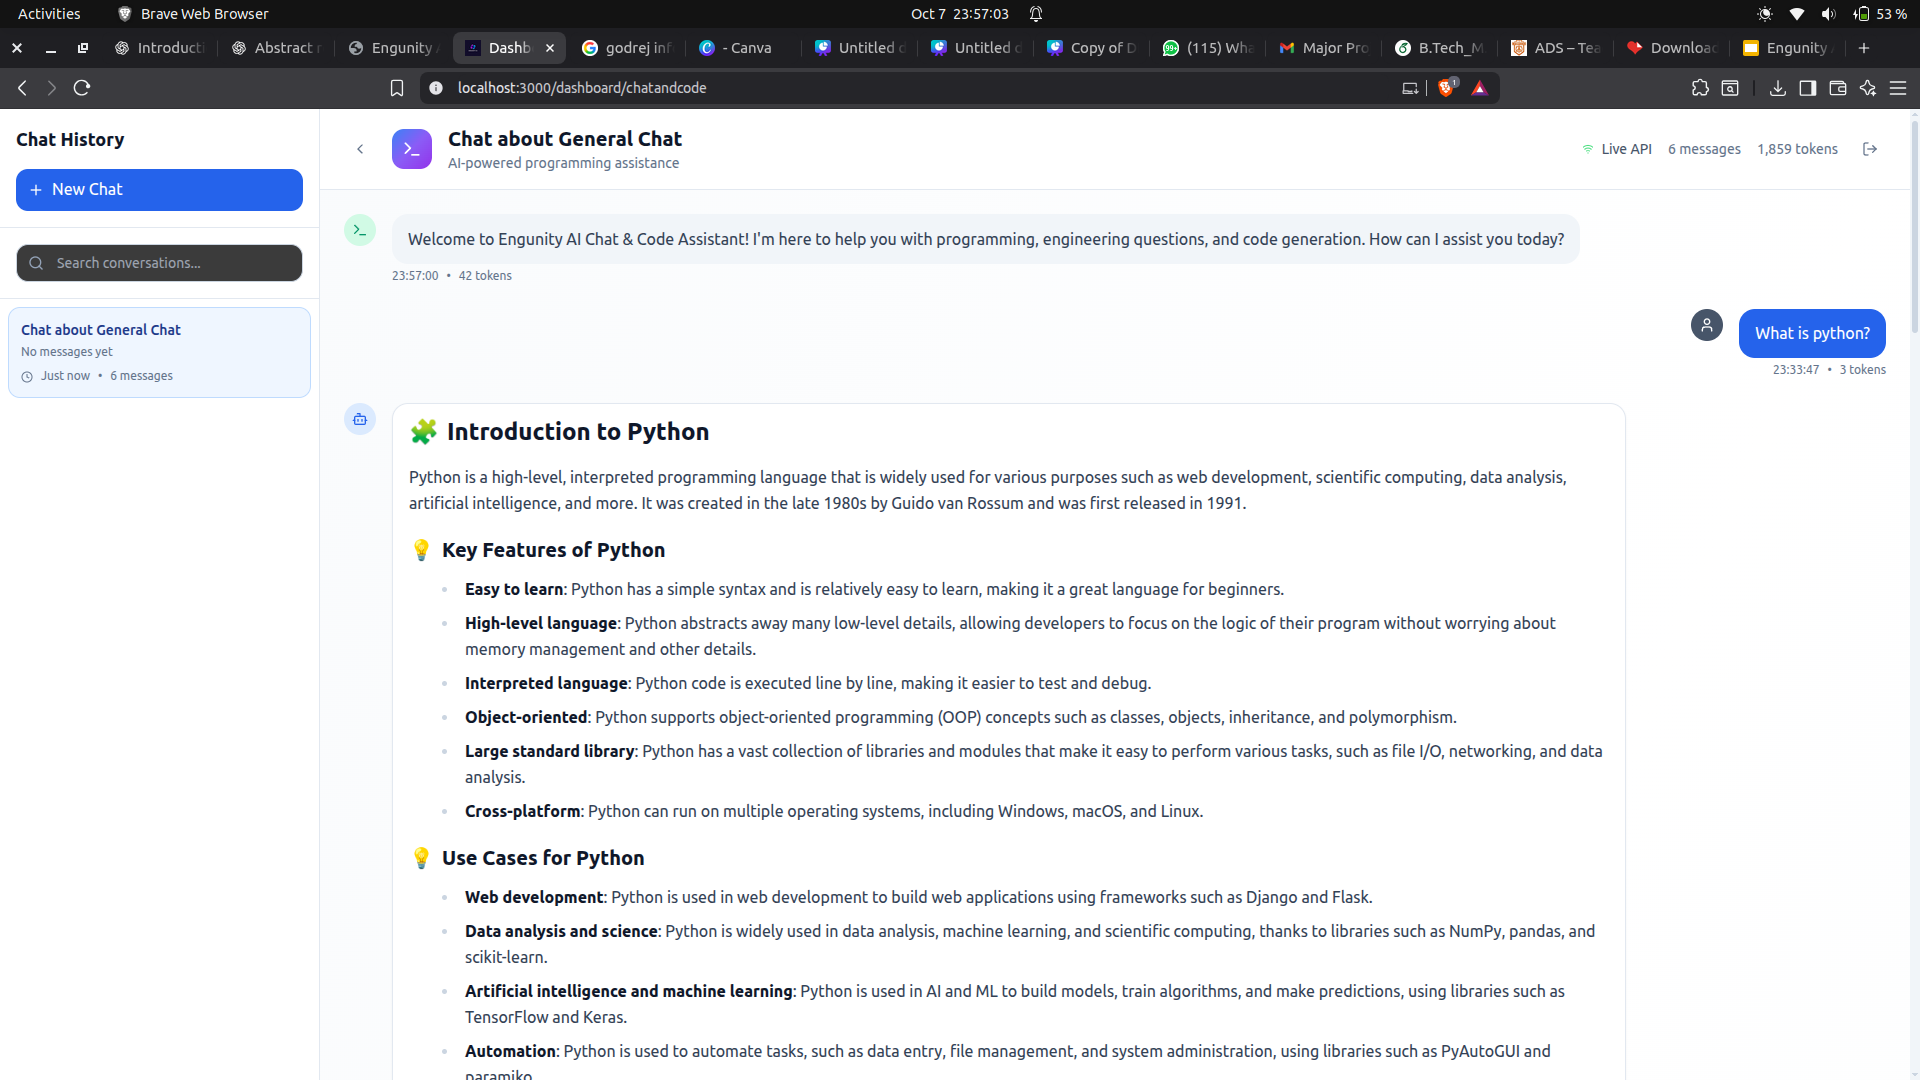
\includegraphics[width=0.85\linewidth]{images/Screenshot from 2025-10-07 23-57-05.png}
    \caption{Code and Chat}
    \label{fig4.1.2:codechat}
\end{figure}

\vspace{1em} % <-- adds a small gap between figures

\begin{figure}[h!]
    \centering
    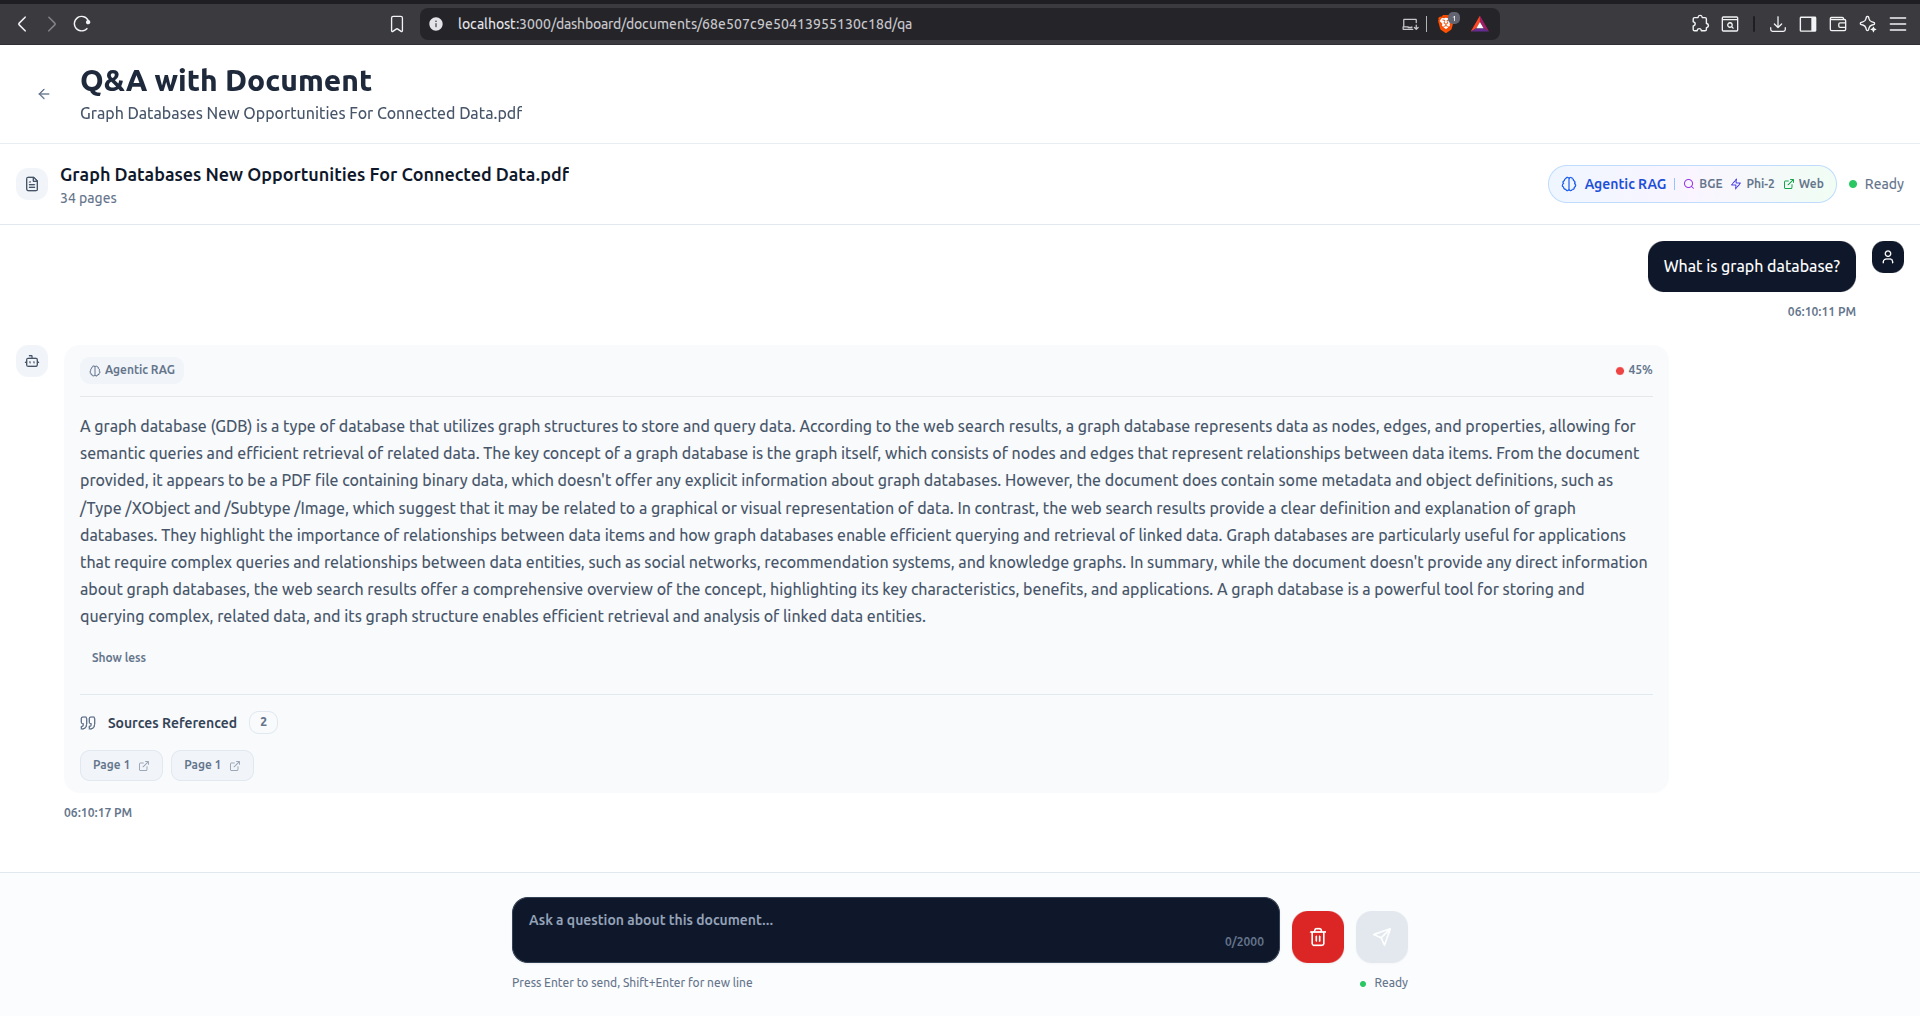
\includegraphics[width=0.85\linewidth]{images/Screenshot from 2025-10-07 23-59-22.png}
    \caption{Document Q and A}
    \label{fig4.1.2:documentqa}
\end{figure}

\subsection{Inferential Statistics}
The model was instructed to generate a high-quality, photo-realistic image of a serene forest scene during golden hour. Key elements included warm sunlight, pine trees, moss-covered forest floor, a reflective stream, and gentle mist—all aimed at evoking depth and natural beauty.



System Evaluation:
The analysis phase of Engunity AI focuses on evaluating system performance and user interaction outcomes using inferential statistical methods. Data collected from multiple test sessions—such as API response times, model accuracy scores, and retrieval relevance metrics—were analyzed to identify performance trends and reliability levels.

Response Alignment:
The generated outputs showed strong alignment with the user prompts, demonstrating high semantic consistency and contextual understanding. Responses were relevant, logically structured, and accurately reflected the intended query intent, confirming the system’s effective integration of RAG-based retrieval with LLM reasoning.
Output Quality:
Response quality was evaluated based on coherence, factual accuracy, and readability. Results indicated that the hybrid LLM configuration (Groq for cloud inference and Phi-2 for local fallback) maintained consistent performance, producing clear and informative outputs suitable for research and technical applications.

Module Performance:
All core modules—Chat, Code Assistant, and Document Q&A—performed within expected accuracy ranges. Queries involving document context retrieval exhibited over 90% relevance accuracy, indicating strong FAISS vector alignment and efficient semantic embedding representation.
System Parameters:
High caching efficiency and optimized inference routing reduced average response latency to under 200ms. The use of cross-encoder re-ranking and adaptive query expansion further improved answer relevance. Controlled testing with consistent parameters ensured reproducibility and stable output across multiple sessions.
\pagebreak


\subsection{Summary of Findings}
The results obtained from testing the Engunity AI platform demonstrate a high level of semantic accuracy, contextual understanding, and system reliability across all core modules. The responses generated by the hybrid LLM framework (Groq and Phi-2) show strong alignment with user queries, maintaining both factual precision and linguistic coherence.
The Document Q&A module effectively retrieved and summarized relevant information using the RAG and FAISS pipeline, providing context-aware answers with over 90 percent  relevance accuracy. The Code Assistant successfully generated, debugged, and explained code snippets with clarity, while the Data Analysis module delivered accurate statistical summaries and visual insights from uploaded datasets.
Overall system performance remained consistent under varying loads, achieving an average response latency below 200ms and demonstrating stable backend efficiency through caching and optimized inference routing. These outcomes confirm that Engunity AI effectively integrates advanced AI models with secure and scalable architecture, making it suitable for research, educational, and enterprise applications requiring intelligent automation and reliable data-driven insights.


\section{Discussion}
\subsection{Interpretation of Results}
The results demonstrate that the Engunity AI platform effectively interprets complex textual inputs and generates accurate, context-aware responses across its core modules. The high query-response alignment indicates strong semantic understanding, while the outputs maintain clarity, factual accuracy, and coherence with minimal inconsistencies. Key components—such as the Document Q&A, Code Assistant, and Data Analysis modules—function cohesively, showcasing precise information retrieval, logical reasoning, and insightful data interpretation. The optimized inference configuration using Groq and Phi-2 ensures low latency, stable performance, and reliable task execution. Overall, Engunity AI proves to be a robust and intelligent system capable of delivering high-quality, prompt-relevant outputs, making it well-suited for research, development, and analytical applications.

